\documentclass[tikz, border=5mm, 12pt]{standalone}
\usepackage{amsmath}
\usepackage{amsfonts}

\usetikzlibrary{arrows.meta,shadows,positioning,calc,decorations.markings}

\pgfdeclarelayer{timelines}
\pgfsetlayers{timelines,main}

\begin{document}

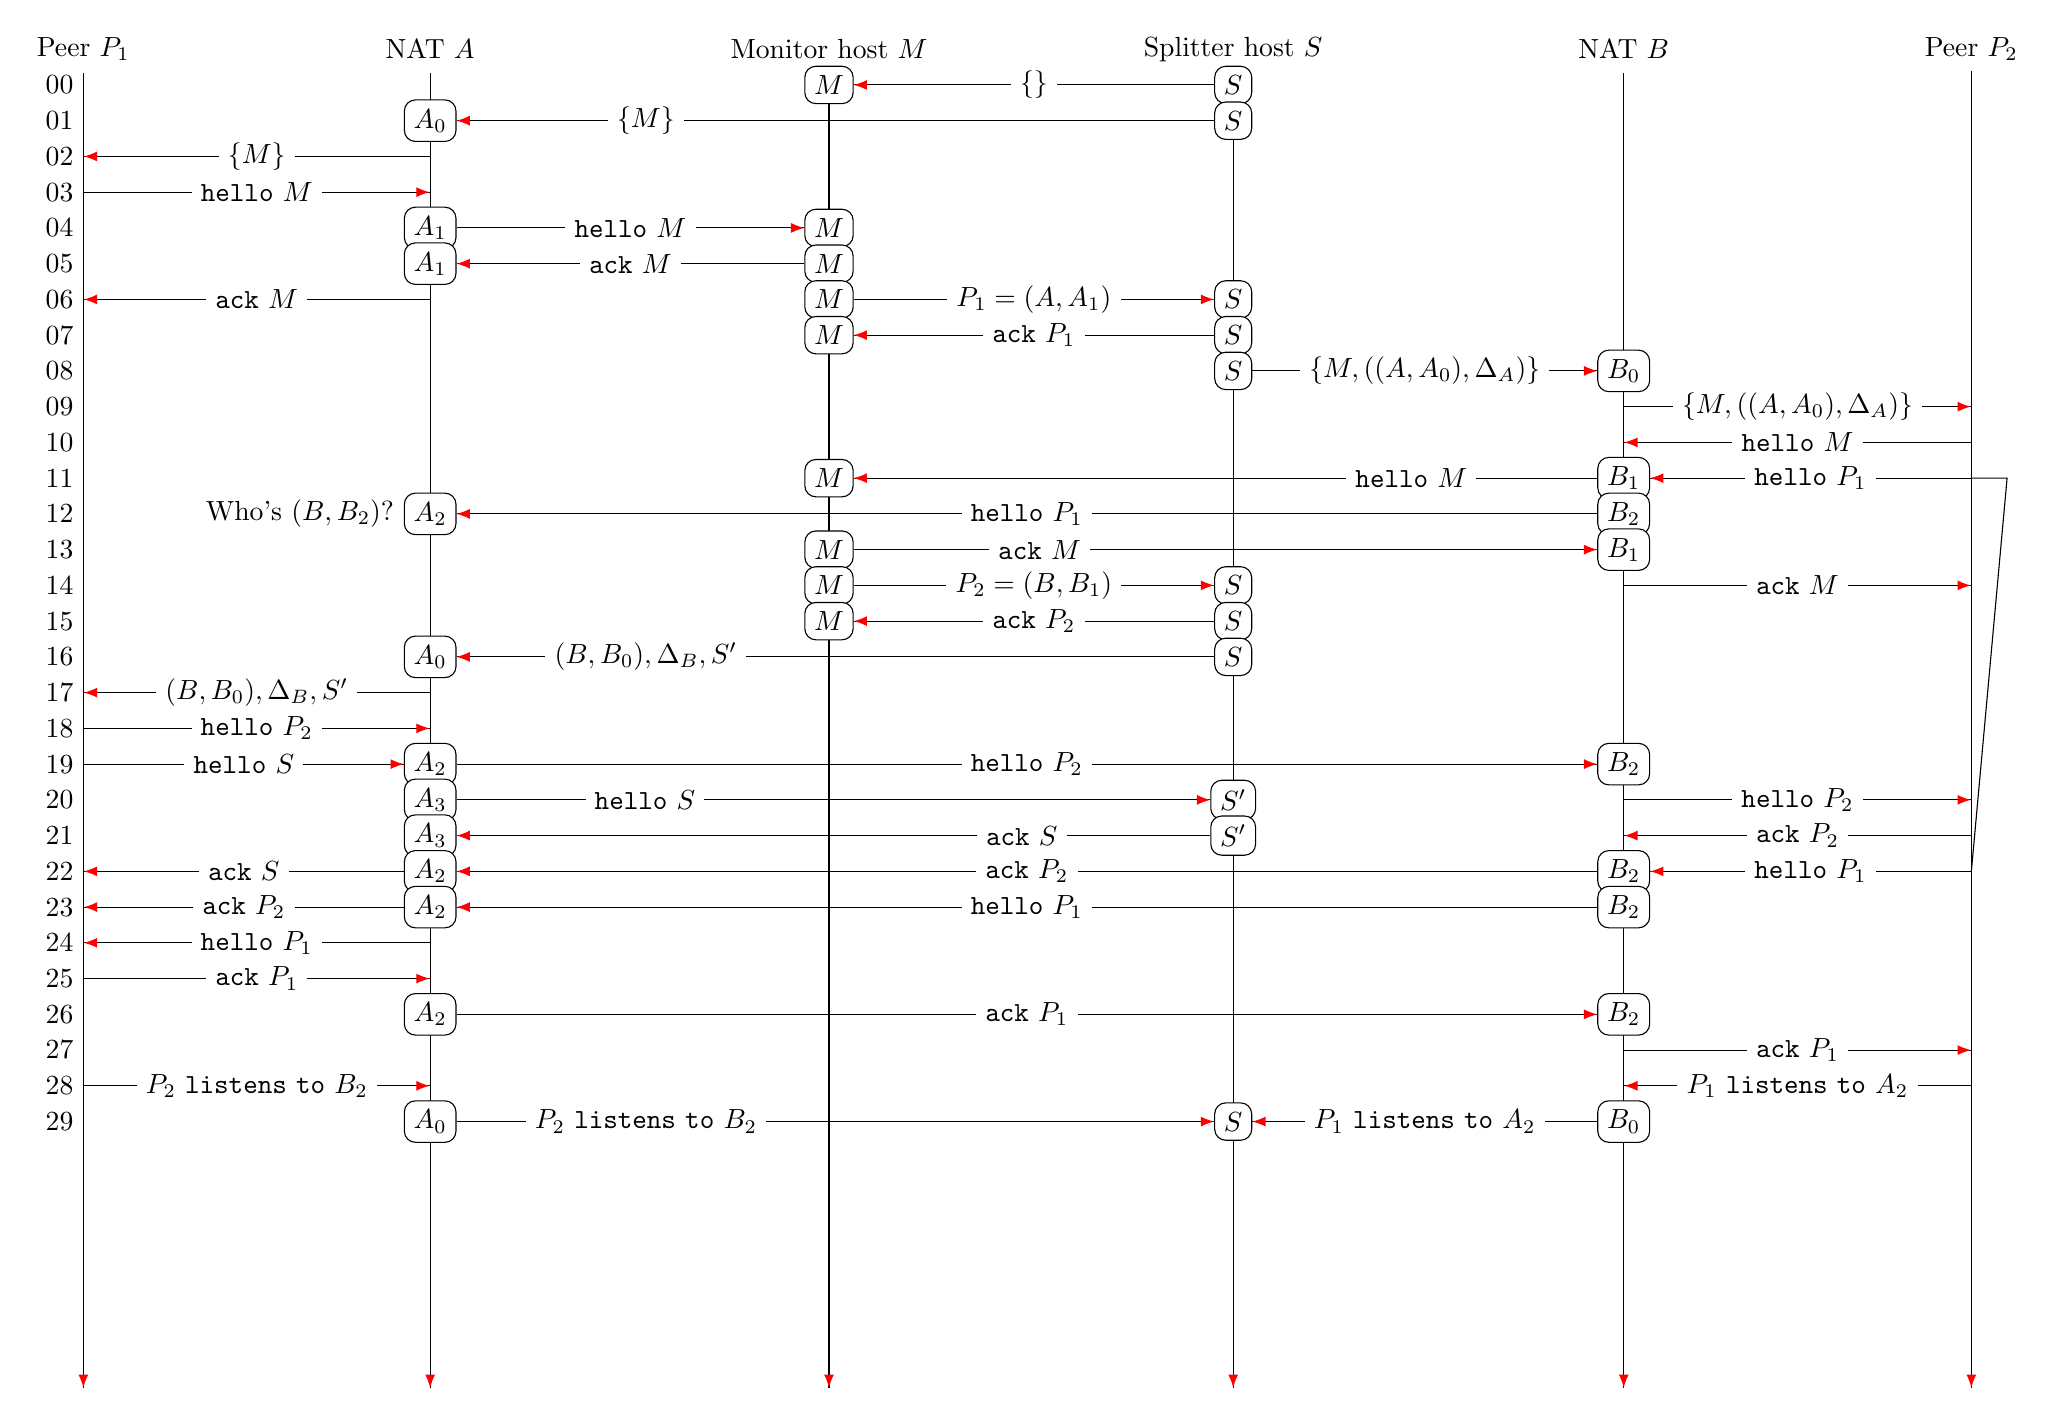
\begin{tikzpicture}
  
  \tikzset{myptr/.style={decoration={markings,mark=at position 1 with %
        {\arrow[red,scale=1.0,>=Latex]{>}}},postaction={decorate}}}
  
  % Entities
  \node[] (Peer A) {Peer $P_1$};
  \node[right=3 of Peer A] (NAT A) {NAT $A$};
  \node[right=3 of NAT A] (Monitor) {Monitor host $M$};
  \node[right=2.5 of Monitor] (Splitter) {Splitter host $S$};
  \node[right=3 of Splitter] (NAT B) {NAT $B$};
  \node[right=3 of NAT B] (Peer B) {Peer $P_2$};

  % Timelines
  \begin{pgfonlayer}{timelines}
    \coordinate (PA) at ($(Peer A.center) + (0.0,-17)$);
    \draw[myptr] ($(Peer A.center) + (0,-2ex)$) -- (PA);  
    \coordinate (NA) at ($(NAT A.center) + (0.0,-17)$);
    \draw[myptr] ($(NAT A.center) + (0,-2ex)$) -- (NA);
    \coordinate (M) at ($(Monitor.center) + (0.0,-17)$);
    \draw[myptr] ($(Monitor.center) + (0,-2ex)$) -- (M);
    \coordinate (S) at ($(Splitter.center) + (0.0,-17)$);
    \draw[myptr] ($(Splitter.center) + (0,-2ex)$) -- (S);
    \coordinate (NB) at ($(NAT B.center) + (0.0,-17)$);
    \draw[myptr] ($(NAT B.center) + (0,-2ex)$) -- (NB);
    \coordinate (PB) at ($(Peer B.center) + (0.0,-17)$);
    \draw[myptr] (Peer B) -- (PB);
  \end{pgfonlayer}
  
  % Time steps
  
  % 00
  \node (00) at ($(Peer A) + (-2ex,-3ex)$) {00};
  \node (S00) at ($(Splitter) + (0,-3ex)$) [fill=white!100,draw,rounded corners] {$S$};
  \node (M00) at ($(Monitor) + (0,-3ex)$) [fill=white!100,draw,rounded corners] {$M$};
  \draw[myptr] (S00) -- (M00) node [pos=0.5,fill=white!100] {\{\}};
  
  % 01
  \node (01) at ($(00) + (0,-3ex)$) {01};
  \path let \p{Splitter}=(Splitter),\p{01}=(01) in node (S01) at (\x{Splitter},\y{01}) [fill=white!100,draw,rounded corners] {$S$};
  \path let \p{NAT A}=(NAT A),\p{01}=(01) in node (NATA01) at (\x{NAT A},\y{01}) [fill=white!100,draw,rounded corners] {$A_0$};
  \draw[myptr] (S01) -- (NATA01) node [pos=0.75,fill=white!100] {$\{M\}$};

  % 02
  \node (02) at ($(01) + (0,-3ex)$) {02};
  \path let \p{NAT A}=(NAT A),\p{02}=(02) in node (NA02) at (\x{NAT A},\y{02}) [inner sep=0pt,minimum size=0pt] {};
  \path let \p{Peer A}=(Peer A),\p{02}=(02) in node (PA02) at (\x{Peer A},\y{02}) [inner sep=0pt,minimum size=0pt] {};
  \draw[myptr] (NA02) -- (PA02) node [pos=0.5,fill=white!100] {$\{M\}$};

  % 03
  \node (03) at ($(02) + (0,-3ex)$) {03};
  \path let \p{03}=(03),\p{Peer A}=(Peer A) in node (PA03) at (\x{Peer A},\y{03}) [inner sep=0pt,minimum size=0pt] {};  
  \path let \p{03}=(03),\p{NAT A}=(NAT A) in node (NA03) at (\x{NAT A},\y{03}) [inner sep=0pt,minimum size=0pt] {};
  \draw[myptr] (PA03) -- (NA03) node [pos=0.5,fill=white!100] {$\mathtt{hello}~M$};
  
  % 04
  \node (04) at ($(03) + (0,-3ex)$) {04};
  \path let \p{04}=(04),\p{NAT A}=(NAT A) in node (N04) at (\x{NAT A},\y{04}) [fill=white!100,draw,rounded corners] {$A_1$};
  \path let \p{04}=(04),\p{Monitor}=(Monitor) in node (M04) at (\x{Monitor},\y{04}) [fill=white!100,draw,rounded corners] {$M$};
  \draw[myptr] (N04) -- (M04) node [pos=0.5,fill=white!100] {$\mathtt{hello}~M$};

  % 05
  \node (05) at ($(04) + (0,-3ex)$) {05};
  \path let \p{Monitor}=(Monitor),\p{05}=(05) in node (M05) at (\x{Monitor},\y{05}) [fill=white!100,draw,rounded corners] {$M$};
  \path let \p{NAT A}=(NAT A),\p{05}=(05) in node (N05) at (\x{NAT A},\y{05}) [fill=white!100,draw,rounded corners] {$A_1$};
  \draw[myptr] (M05) -- (N05) node [pos=0.5,fill=white!100] {$\mathtt{ack}~M$};

  % 06
  \node (06) at ($(05) + (0,-3ex)$) {06};
  \path let \p{NAT A}=(NAT A),\p{06}=(06) in node (NA06) at (\x{NAT A},\y{06}) [inner sep=0pt,minimum size=0pt] {};
  \path let \p{Peer A}=(Peer A),\p{06}=(06) in node (PA06) at (\x{Peer A},\y{06}) [inner sep=0pt,minimum size=0pt] {};
  \draw[myptr] (NA06) -- (PA06) node [pos=0.5,fill=white!100] {$\mathtt{ack}~M$};
  \path let \p{Splitter}=(Splitter),\p{06}=(06) in node (S06) at (\x{Splitter},\y{06}) [fill=white!100,draw,rounded corners] {$S$};
  \path let \p{Monitor}=(Monitor),\p{06}=(06) in node (M06) at (\x{Monitor},\y{06}) [fill=white!100,draw,rounded corners] {$M$};
  \draw[myptr] (M06) -- (S06) node [pos=0.5,fill=white!100] {$P_1=(A,A_1)$};
  
  % 07
  \node (07) at ($(06) + (0,-3ex)$) {07};
  \path let \p{Monitor}=(Monitor),\p{07}=(07) in node (M07) at (\x{Monitor},\y{07}) [fill=white!100,draw,rounded corners] {$M$};
  \path let \p{Splitter}=(Splitter),\p{07}=(07) in node (S07) at (\x{Splitter},\y{07}) [fill=white!100,draw,rounded corners] {$S$};
  \draw[myptr] (S07) -- (M07) node [pos=0.5,fill=white!100] {$\mathtt{ack}~P_1$};

  % 08
  \node (08) at ($(07) + (0,-3ex)$) {08};
  \path let \p{Splitter}=(Splitter),\p{08}=(08) in node (S08) at (\x{Splitter},\y{08}) [fill=white!100,draw,rounded corners] {$S$};
  \path let \p{NAT B}=(NAT B),\p{08}=(08) in node (NB08) at (\x{NAT B},\y{08}) [fill=white!100,draw,rounded corners] {$B_0$};
  \draw[myptr] (S08) -- (NB08) node [pos=0.5,fill=white!100] {$\{M,((A,A_0),\Delta_A)\}$};
  
  % 09
  \node (09) at ($(08) + (0,-3ex)$) {09};
  \path let \p{NAT B}=(NAT B),\p{09}=(09) in node (NB09) at (\x{NAT B},\y{09}) [inner sep=0pt,minimum size=0pt] {};
  \path let \p{Peer B}=(Peer B),\p{09}=(09) in node (PB09) at (\x{Peer B},\y{09}) [inner sep=0pt,minimum size=0pt] {};
  \draw[myptr] (NB09) -- (PB09) node [pos=0.5,fill=white!100] {$\{M,((A,A_0),\Delta_A)\}$};
  
  % 10
  \node (10) at ($(09) + (0,-3ex)$) {10};
  \path let \p{Peer B}=(Peer B),\p{10}=(10) in node (PB10) at (\x{Peer B},\y{10}) [inner sep=0pt,minimum size=0pt] {};
  \path let \p{NAT B}=(NAT B),\p{10}=(10) in node (NB10) at (\x{NAT B},\y{10}) [inner sep=0pt,minimum size=0pt] {};
  \draw[myptr] (PB10) -- (NB10) node [pos=0.5,fill=white!100] {$\mathtt{hello}~M$};
  
  % 11
  \node (11) at ($(10) + (0,-3ex)$) {11};
  \path let \p{NAT B}=(NAT B),\p{11}=(11) in node (NB11) at (\x{NAT B},\y{11}) [fill=white!100,draw,rounded corners] {$B_1$};
  \path let \p{Monitor}=(Monitor),\p{11}=(11) in node (M11) at (\x{Monitor},\y{11}) [fill=white!100,draw,rounded corners] {$M$};
  \draw[myptr] (NB11) -- (M11) node [pos=0.25,fill=white!100] {$\mathtt{hello}~M$};
  \path let \p{Peer B}=(Peer B),\p{11}=(11) in node (PB11) at (\x{Peer B},\y{11}) [inner sep=0pt,minimum size=0pt] {};
  \draw[myptr] (PB11) -- (NB11) node [pos=0.5,fill=white!100] {$\mathtt{hello}~P_1$};
  
  % 12
  \node (12) at ($(11) + (0,-3ex)$) {12};
  \path let \p{NAT B}=(NAT B),\p{12}=(12) in node (NB12) at (\x{NAT B},\y{12}) [fill=white!100,draw,rounded corners] {$B_2$};
  \path let \p{NAT A}=(NAT A),\p{12}=(12) in node (NA12) at (\x{NAT A},\y{12}) [fill=white!100,draw,rounded corners] {$A_2$};
  \draw[myptr] (NB12) -- (NA12) node [pos=0.5,fill=white!100] {$\mathtt{hello}~P_1$};
  \node [left=0 of NA12] {Who's $(B,B_2)$?};

  % 13
  \node (13) at ($(12) + (0,-3ex)$) {13};
  \path let \p{Monitor}=(Monitor),\p{13}=(13) in node (M13) at (\x{Monitor},\y{13}) [fill=white!100,draw,rounded corners] {$M$};
  \path let \p{NAT B}=(NAT B),\p{13}=(13) in node (NB13) at (\x{NAT B},\y{13}) [fill=white!100,draw,rounded corners] {$B_1$};
  \draw[myptr] (M13) -- (NB13) node [pos=0.25,fill=white!100] {$\mathtt{ack}~M$};

  % 14
  \node (14) at ($(13) + (0,-3ex)$) {14};
  \path let \p{Monitor}=(Monitor),\p{14}=(14) in node (M14) at (\x{Monitor},\y{14}) [fill=white!100,draw,rounded corners] {$M$};
  \path let \p{Splitter}=(Splitter),\p{14}=(14) in node (S14) at (\x{Splitter},\y{14}) [fill=white!100,draw,rounded corners] {$S$};
  \draw[myptr] (M14) -- (S14) node [pos=0.5,fill=white!100] {$P_2=(B,B_1)$};
  \path let \p{NAT B}=(NAT B),\p{14}=(14) in node (NB14) at (\x{NAT B},\y{14}) [inner sep=0pt,minimum size=0pt] {};
  \path let \p{Peer B}=(Peer B),\p{14}=(14) in node (PB14) at (\x{Peer B},\y{14}) [inner sep=0pt,minimum size=0pt] {};
  \draw[myptr] (NB14) -- (PB14) node [pos=0.5,fill=white!100] {$\mathtt{ack}~M$};
  
  % 15
  \node (15) at ($(14) + (0,-3ex)$) {15};
  \path let \p{Splitter}=(Splitter),\p{15}=(15) in node (S15) at (\x{Splitter},\y{15}) [fill=white!100,draw,rounded corners] {$S$};
  \path let \p{Monitor}=(Monitor),\p{15}=(15) in node (M15) at (\x{Monitor},\y{15}) [fill=white!100,draw,rounded corners] {$M$};
  \draw[myptr] (S15) -- (M15) node [pos=0.5,fill=white!100] {$\mathtt{ack}~P_2$};

  % 16
  \node (16) at ($(15) + (0,-3ex)$) {16};
  \path let \p{Splitter}=(Splitter),\p{16}=(16) in node (S16) at (\x{Splitter},\y{16}) [fill=white!100,draw,rounded corners] {$S$};
  \path let \p{NAT A}=(NAT A),\p{16}=(16) in node (NA16) at (\x{NAT A},\y{16}) [fill=white!100,draw,rounded corners] {$A_0$};
  \draw[myptr] (S16) -- (NA16) node [pos=0.75,fill=white!100] {$(B,B_0),\Delta_B,S'$};

  % 17
  \node (17) at ($(16) + (0,-3ex)$) {17};
  \path let \p{NAT A}=(NAT A),\p{17}=(17) in node (NA17) at (\x{NAT A},\y{17}) [inner sep=0pt,minimum size=0pt] {};
  \path let \p{Peer A}=(Peer A),\p{17}=(17) in node (PA17) at (\x{Peer A},\y{17}) [inner sep=0pt,minimum size=0pt] {};
  \draw[myptr] (NA17) -- (PA17) node [pos=0.50,fill=white!100] {$(B,B_0),\Delta_B,S'$};

  % 18
  \node (18) at ($(17) + (0,-3ex)$) {18};
  \path let \p{Peer A}=(Peer A),\p{18}=(18) in node (PA18) at (\x{Peer A},\y{18}) [inner sep=0pt,minimum size=0pt] {};
  \path let \p{NAT A}=(NAT A),\p{18}=(18) in node (NA18) at (\x{NAT A},\y{18}) [inner sep=0pt,minimum size=0pt] {};
  \draw[myptr] (PA18) -- (NA18) node [pos=0.50,fill=white!100] {$\mathtt{hello}~P_2$};

  % 19
  \node (19) at ($(18) + (0,-3ex)$) {19};
  \path let \p{Peer A}=(Peer A),\p{19}=(19) in node (PA19) at (\x{Peer A},\y{19}) [inner sep=0pt,minimum size=0pt] {};
  \path let \p{NAT A}=(NAT A),\p{19}=(19) in node (NA19) at (\x{NAT A},\y{19}) [fill=white!100,draw,rounded corners] {$A_2$};
  \draw[myptr] (PA19) -- (NA19) node [pos=0.50,fill=white!100] {$\mathtt{hello}~S$};
  \path let \p{NAT B}=(NAT B),\p{19}=(19) in node (NB19) at (\x{NAT B},\y{19}) [fill=white!100,draw,rounded corners] {$B_2$};
  \draw[myptr] (NA19) -- (NB19) node [pos=0.5,fill=white!100] {$\mathtt{hello}~P_2$};
  
  % 20
  \node (20) at ($(19) + (0,-3ex)$) {20};
  \path let \p{NAT A}=(NAT A),\p{20}=(20) in node (NA20) at (\x{NAT A},\y{20}) [fill=white!100,draw,rounded corners] {$A_3$};
  \path let \p{Splitter}=(Splitter),\p{20}=(20) in node (S20) at (\x{Splitter},\y{20}) [fill=white!100,draw,rounded corners] {$S'$};
  \draw[myptr] (NA20) -- (S20) node [pos=0.25,fill=white!100] {$\mathtt{hello}~S$};
  \path let \p{NAT B}=(NAT B),\p{20}=(20) in node (NB20) at (\x{NAT B},\y{20}) [inner sep=0pt,minimum size=0pt] {};
  \path let \p{Peer B}=(Peer B),\p{20}=(20) in node (PB20) at (\x{Peer B},\y{20}) [inner sep=0pt,minimum size=0pt] {};
  \draw[myptr] (NB20) -- (PB20) node [pos=0.5,fill=white!100] {$\mathtt{hello}~P_2$};

  % 21
  \node (21) at ($(20) + (0,-3ex)$) {21};
  \path let \p{Splitter}=(Splitter),\p{21}=(21) in node (S21) at (\x{Splitter},\y{21}) [fill=white!100,draw,rounded corners] {$S'$};
  \path let \p{NAT A}=(NAT A),\p{21}=(21) in node (NA21) at (\x{NAT A},\y{21}) [fill=white!100,draw,rounded corners] {$A_3$};
  \draw[myptr] (S21) -- (NA21) node [pos=0.25,fill=white!100] {$\mathtt{ack}~S$};
  \path let \p{Peer B}=(Peer B),\p{21}=(21) in node (PB21) at (\x{Peer B},\y{21}) [inner sep=0pt,minimum size=0pt] {};
  \path let \p{NAT B}=(NAT B),\p{21}=(21) in node (NB21) at (\x{NAT B},\y{21}) [inner sep=0pt,minimum size=0pt] {};
  \draw[myptr] (PB21) -- (NB21) node [pos=0.5,fill=white!100] {$\mathtt{ack}~P_2$};

  % 22
  \node (22) at ($(21) + (0,-3ex)$) {22};
  \path let \p{NAT A}=(NAT A),\p{22}=(22) in node (NA22) at (\x{NAT A},\y{22}) [fill=white!100,draw,rounded corners] {$A_2$};
  \path let \p{Peer A}=(Peer A),\p{22}=(22) in node (PA22) at (\x{Peer A},\y{22}) [inner sep=0pt,minimum size=0pt] {};
  \draw[myptr] (NA22) -- (PA22) node [pos=0.50,fill=white!100] {$\mathtt{ack}~S$};
  \path let \p{NAT B}=(NAT B),\p{22}=(22) in node (NB22) at (\x{NAT B},\y{22}) [fill=white!100,draw,rounded corners] {$B_2$};
  \draw[myptr] (NB22) -- (NA22) node [pos=0.5,fill=white!100] {$\mathtt{ack}~P_2$};
  \path let \p{Peer B}=(Peer B),\p{22}=(22) in node (PB22) at (\x{Peer B},\y{22}) [inner sep=0pt,minimum size=0pt] {};
  \draw[myptr] (PB22) -- (NB22) node [pos=0.5,fill=white!100] {$\mathtt{hello}~P_1$};

  % 23
  \node (23) at ($(22) + (0,-3ex)$) {23};
  \path let \p{NAT A}=(NAT A),\p{23}=(23) in node (NA23) at (\x{NAT A},\y{23}) [fill=white!100,draw,rounded corners] {$A_2$};
  \path let \p{Peer A}=(Peer A),\p{23}=(23) in node (PA23) at (\x{Peer A},\y{23}) [inner sep=0pt,minimum size=0pt] {};
  \draw[myptr] (NA23) -- (PA23) node [pos=0.50,fill=white!100] {$\mathtt{ack}~P_2$};
  \path let \p{NAT B}=(NAT B),\p{23}=(23) in node (NB23) at (\x{NAT B},\y{23}) [fill=white!100,draw,rounded corners] {$B_2$};
  \draw[myptr] (NB23) -- (NA23) node [pos=0.5,fill=white!100] {$\mathtt{hello}~P_1$};

  % 24
  \node (24) at ($(23) + (0,-3ex)$) {24};
  \path let \p{NAT A}=(NAT A),\p{24}=(24) in node (NA24) at (\x{NAT A},\y{24}) [inner sep=0pt,minimum size=0pt] {};
  \path let \p{Peer A}=(Peer A),\p{24}=(24) in node (PA24) at (\x{Peer A},\y{24}) [inner sep=0pt,minimum size=0pt] {};
  \draw[myptr] (NA24) -- (PA24) node [pos=0.5,fill=white!100] {$\mathtt{hello}~P_1$};

  % 25
  \node (25) at ($(24) + (0,-3ex)$) {25};
  \path let \p{Peer A}=(Peer A),\p{25}=(25) in node (PA25) at (\x{Peer A},\y{25}) [inner sep=0pt,minimum size=0pt] {};
  \path let \p{NAT A}=(NAT A),\p{25}=(25) in node (NA25) at (\x{NAT A},\y{25}) [inner sep=0pt,minimum size=0pt] {};
  \draw[myptr] (PA25) -- (NA25) node [pos=0.5,fill=white!100] {$\mathtt{ack}~P_1$};

  % 26
  \node (26) at ($(25) + (0,-3ex)$) {26};
  \path let \p{NAT A}=(NAT A),\p{26}=(26) in node (NA26) at (\x{NAT A},\y{26}) [fill=white!100,draw,rounded corners] {$A_2$};
  \path let \p{NAT B}=(NAT B),\p{26}=(26) in node (NB26) at (\x{NAT B},\y{26}) [fill=white!100,draw,rounded corners] {$B_2$};
  \draw[myptr] (NA26) -- (NB26) node [pos=0.5,fill=white!100] {$\mathtt{ack}~P_1$};

  % 27
  \node (27) at ($(26) + (0,-3ex)$) {27};
  \path let \p{NAT B}=(NAT B),\p{27}=(27) in node (NB27) at (\x{NAT B},\y{27}) [inner sep=0pt,minimum size=0pt] {};
  \path let \p{Peer B}=(Peer B),\p{27}=(27) in node (PB27) at (\x{Peer B},\y{27}) [inner sep=0pt,minimum size=0pt] {};
  \draw[myptr] (NB27) -- (PB27) node [pos=0.5,fill=white!100] {$\mathtt{ack}~P_1$};

  % 28
  \node (28) at ($(27) + (0,-3ex)$) {28};
  \path let \p{Peer A}=(Peer A),\p{28}=(28) in node (PA28) at (\x{Peer A},\y{28}) [inner sep=0pt,minimum size=0pt] {};
  \path let \p{NAT A}=(NAT A),\p{28}=(28) in node (NA28) at (\x{NAT A},\y{28}) [inner sep=0pt,minimum size=0pt] {};
  \draw[myptr] (PA28) -- (NA28) node [pos=0.50,fill=white!100] {$P_2~\mathtt{listens~to}~B_2$};
  \path let \p{Peer B}=(Peer B),\p{28}=(28) in node (PB28) at (\x{Peer B},\y{28}) [inner sep=0pt,minimum size=0pt] {};
  \path let \p{NAT B}=(NAT B),\p{28}=(28) in node (NB28) at (\x{NAT B},\y{28}) [inner sep=0pt,minimum size=0pt] {};
  \draw[myptr] (PB28) -- (NB28) node [pos=0.5,fill=white!100] {$P_1~\mathtt{listens~to}~A_2$};

  % 29
  \node (29) at ($(28) + (0,-3ex)$) {29};
  \path let \p{NAT A}=(NAT A),\p{29}=(29) in node (NA29) at (\x{NAT A},\y{29}) [fill=white!100,draw,rounded corners] {$A_0$};
  \path let \p{Splitter}=(Splitter),\p{29}=(29) in node (S29) at (\x{Splitter},\y{29}) [fill=white!100,draw,rounded corners] {$S$};
  \draw[myptr] (NA29) -- (S29) node [pos=0.25,fill=white!100] {$P_2~\mathtt{listens~to}~B_2$};
  \path let \p{NAT B}=(NAT B),\p{29}=(29) in node (NB29) at (\x{NAT B},\y{29}) [fill=white!100,draw,rounded corners] {$B_0$};
  \draw[myptr] (NB29) -- (S29) node [pos=0.5,fill=white!100] {$P_1~\mathtt{listens~to}~A_2$};

  \begin{pgfonlayer}{timelines}
    % Timeout PB11 -> PB22
    \coordinate (timeout) at ($(PB11) + (3ex, 0)$);
    \draw (PB11) -- (timeout) -- (PB22);
  \end{pgfonlayer}

\end{tikzpicture}

\end{document}
